\documentclass[portrait]{a0poster}
\usepackage[T1]{fontenc}

\usepackage[english]{babel} % langue utilisée

% \usepackage{lmodern} % For times font (times)
\renewcommand{\familydefault}{\sfdefault}
\usepackage[scaled]{helvet}

\usepackage{titlesec} % pour de plus beaux titres ?
\usepackage{amsmath} %,amsfonts,amsmath,amssymb,amsthm % symboles mathématiques

\usepackage{multicol} % multiples colonnes
\usepackage{float} % float environnement
\usepackage[svgnames]{xcolor} % plus de couleurs
\usepackage[most]{tcolorbox}

\usepackage{graphicx} % add figures and images
\usepackage{caption}
\graphicspath{{./fig/} } % image and figure path
\usepackage{tikz} % pour les graphiques
\usepackage{exscale} % ordre de mesures...

\usepackage[
    sorting=none,
    doi=false,
    url=false,
    isbn=false,
    eprint=false, 
    giveninits=true,
    maxbibnames=1 
]{biblatex} % bibliographie
\AtEveryBibitem{\clearlist{language}}
\addbibresource{biblio.bib}
\def\bibfont{\footnotesize}

%% Reformatage du fichier
\usepackage[left=1cm,right=1cm,top=1cm,bottom=1cm]{geometry}
\setlength{\paperwidth}{90.cm}	% Poster width in cm
\setlength{\paperheight}{90.cm}	% Poster height in cm
\setlength{\textwidth}{87.cm}
\setlength{\textheight}{87.cm}

%% Reformatage des tailles de titre
\titleformat*{\section}{\LARGE\bfseries}
\titleformat*{\subsection}{\Large\bfseries}
\titleformat*{\subsubsection}{\large\bfseries}
\titleformat*{\paragraph}{\large\bfseries}


% %%%%%%%%%%%%%%%%%%%%%%%%%%%%%%%%%%%%%
% %         Début Document            %
% %%%%%%%%%%%%%%%%%%%%%%%%%%%%%%%%%%%%%

\begin{document}
    \begin{minipage}{\textwidth}
        \begin{minipage}{0.62\textwidth}
            \textbf{\Huge Single neuron and population analysis of visual motion direction : effect of uncertaincy.} \vspace{1cm} \\
            \textbf{\large Alexandre Lainé *¹,  Nicholas J. Priebe ², Guillaume S. Masson ¹, Laurent U. Perrinet ¹} \\
            \large ¹ Institut de Neurosciences de la Timone, UMR 7289, CNRS and Aix-Marseille Université, Marseille, 13005, France.\\ 
            \large ² Section of Neurobiology, School of Biological Sciences, University of Texas at Austin, Austin, TX, USA.\\ 
            \large * Correspondence : alexandre.laine@univ-amu.fr
        \end{minipage}
        \hfill
        \begin{minipage}{0.35\textwidth}
            \begin{minipage}{0.48\textwidth}
                
\includegraphics[width=1\textwidth]{LogoAmidex.png} \\
                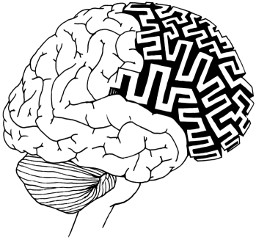
\includegraphics[width=0.35\textwidth]{LogoAREADNE.jpg}
                
\includegraphics[width=0.6\textwidth]{LogoAMU.pdf}
            \end{minipage}
            \hfill
            \begin{minipage}{0.48\textwidth}
                
\includegraphics[width=1\textwidth]{LogoINT.pdf}
            \end{minipage}
        \end{minipage}
    \end{minipage}
    \vspace{0.5cm}

    \begin{minipage}{\textwidth}
        \begin{minipage}{0.42\textwidth}      
            \begin{tcolorbox}[
                enhanced,
                colframe=blue!60!white,
                colback=white,
                boxsep=2mm,
                arc=5mm,
                boxrule=3pt,
                attach boxed title to top left={xshift=8mm,yshift=-3mm},
                boxed title style={
                    colback=white,
                    colframe=white,
                    sharp corners
                },
                coltitle=black,
                title=\textbf{\Large Introduction}
            ]
                \begin{minipage}{\textwidth}
                    \begin{minipage}{0.53\textwidth}
                        Studying the \textbf{internal representation} of natural features in the primary visual cortex (V1), like direction or spatial frequency, is crucial to understand how we perceive the external world. Research on 2D motion direction in \textbf{non-human primates} in particular when displaying  \textbf{naturalist-like stimuli} like Motion-Clouds reveals substantial diversity and multiple mechanisms within the neuronal population~\cite{Ladret_Cortes_Ikan_Chavane_Casanova_Perrinet_2023}. The aim of this project is to examine how a large population of V1 neurons encodes stimulus direction and how this representation is modulated by the uncertainty.

                        \captionof{figure}{\textbf{A.} The aperture problem. \textbf{B.} 1D vs 2D visual information. \textbf{C.} Orientation distribution of natural patches. (\textbf{A} and \textbf{B} are adapted from~\cite{Montagnini_Mamassian_Perrinet_Castet_Masson_2007})}
                    \end{minipage}
                    \hfill
                    \begin{minipage}{0.45\textwidth}
                        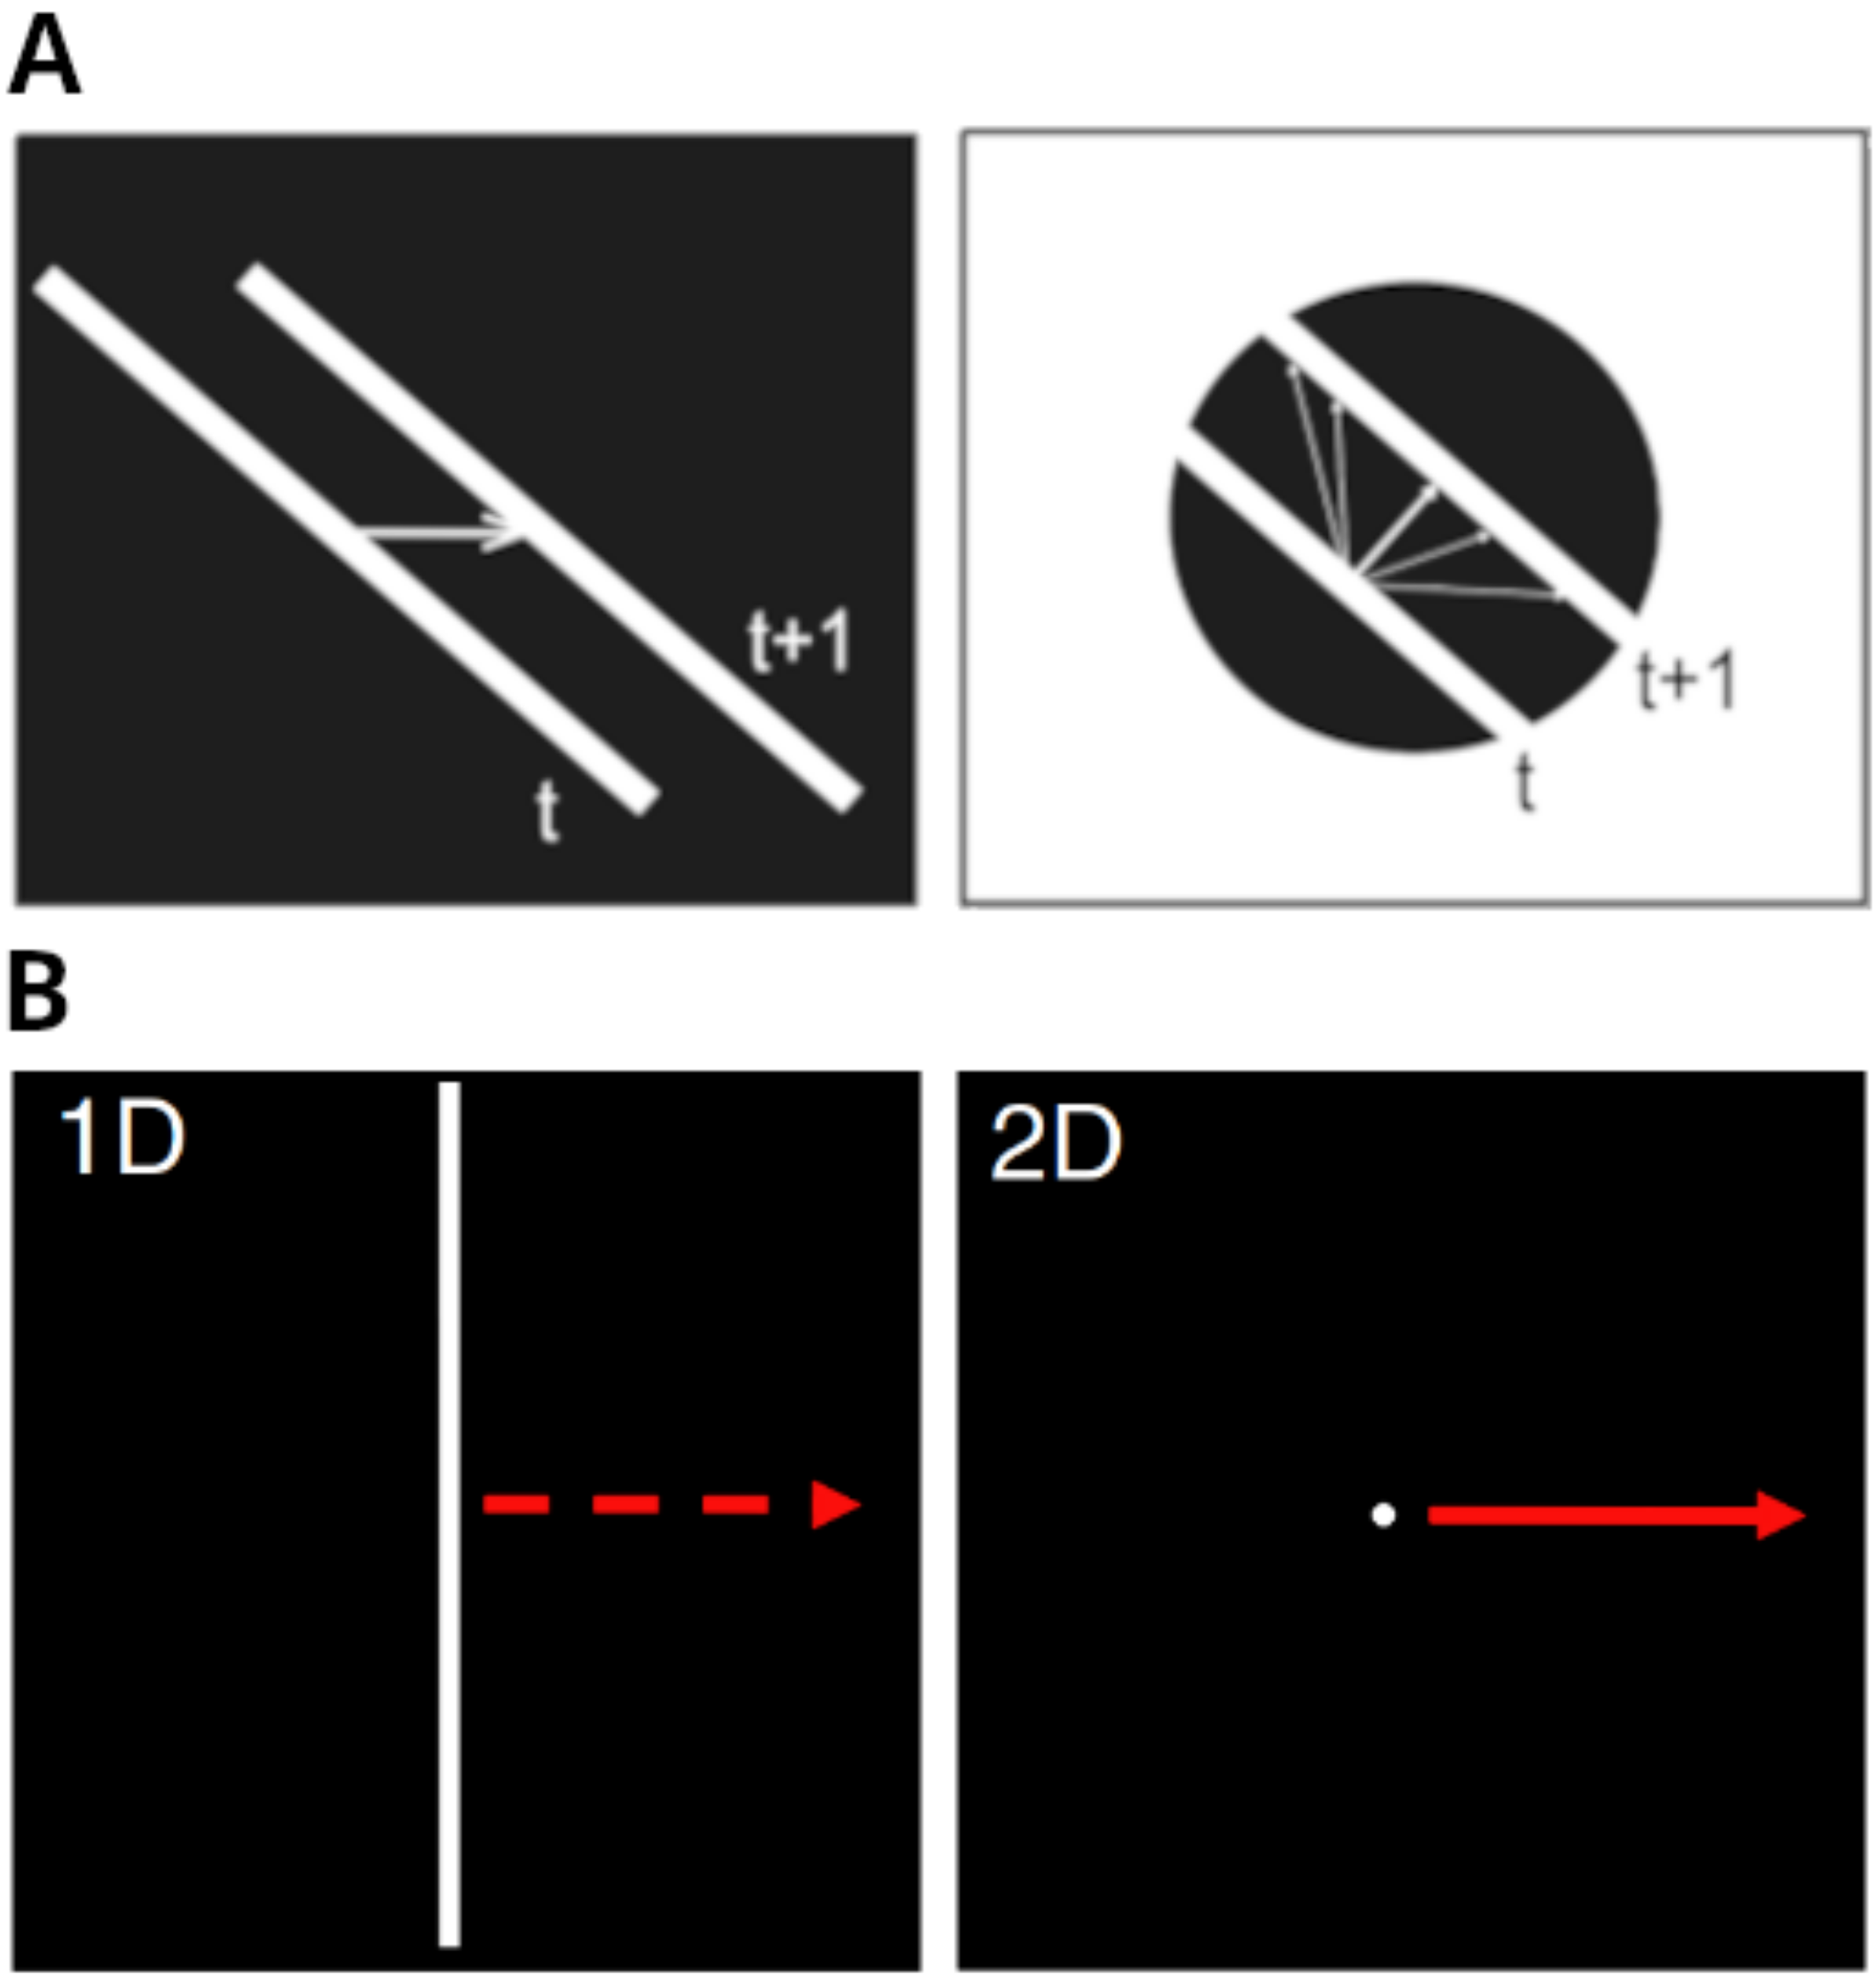
\includegraphics[width=\textwidth]{1D2D_Aperturepb_Montagnini2007.png}
                    \end{minipage}
                \end{minipage}

                \vspace{0.5cm}
                \begin{minipage}{\textwidth}
                    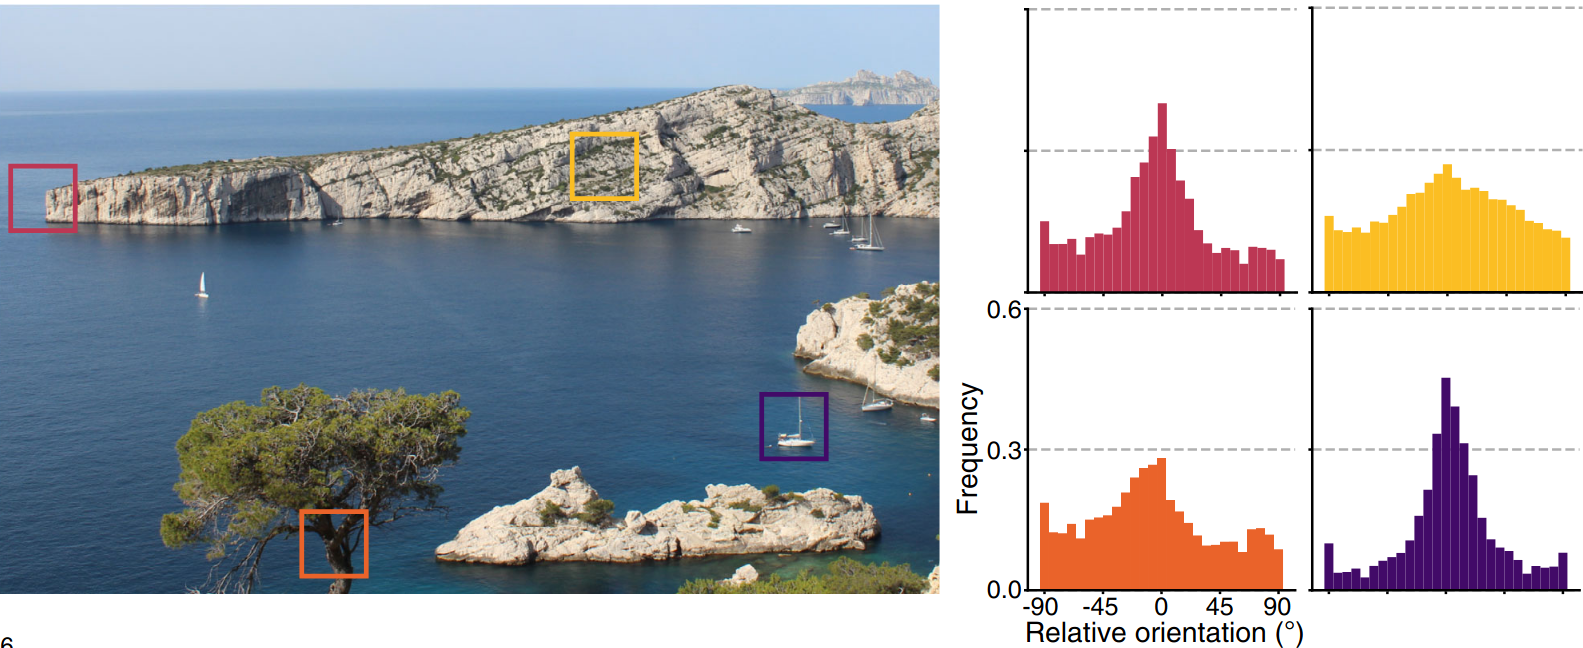
\includegraphics[width=\textwidth]{Intro-Hugo.png}
                \end{minipage}
            \end{tcolorbox}
        \end{minipage}
        \hfill
        \begin{minipage}{0.56\textwidth}
            \begin{tcolorbox}[
                enhanced,
                colframe=red!60!white,
                colback=white,
                arc=3mm,
                boxsep=2mm,
                boxrule=3pt,
                attach boxed title to top left={xshift=8mm,yshift=-3mm},
                boxed title style={
                    colback=white,
                    colframe=white,
                    sharp corners
                },
                coltitle=black,
                title=\textbf{\Large Method}
            ]
                \begin{minipage}{0.39\textwidth}
                    \begin{minipage}{\textwidth}
                        Neuronal recordings were made in V1 of one marmoset monkey using the Neuropixel technology during 2D motion presentation in twelve directions ($\theta$) from $0^{\circ}$ to $330^{\circ}$, four levels of orientation bandwidth ($B_\theta$; $0^{\circ}$, $15^{\circ}$, $30^{\circ}$ and $45^{\circ}$) and four levels of spatial frequency bandwidth ($B_{sf}$; $0.01$, $0.175$, $0.7$ and $2.8$ cpd).
                        A Motion-Clouds~\cite{Leon_Vanzetta_Masson_Perrinet_2012} is obtained by assigning a random phase to its corresponding Fourier envelope and computing the inverse Fourier transform. \\

                        The decoding method based on \cite{Jazayeri_Movshon_2006} defines the likelihood function of the stimulus direction as an equivalent to the sum of the likelihood functions of each neuron, which is equivalent to summing the agreement functions of each neuron weighted by the activity of each neuron during stimulus presentation. \\

                        If we take $W_i$ as the tuning curve of neuron $i$ and $A^s_i$ as the activity induced by simulus $s$. Then, $L^s_i$ and $L^s$ are respectively the likelihood function for a particular trial of the neuron $i$ and the population.

                        \begin{equation*}
                            \log{L^s(\theta)} = \sum^N_{i=0}\log{L^s_i(\theta)} = \sum^N_{i=0}{A^s_i(\theta)\log{W_i(\theta)}}
                        \end{equation*}
                    \end{minipage}
                \end{minipage}
                \hfill
                \begin{minipage}{0.59\textwidth}
                    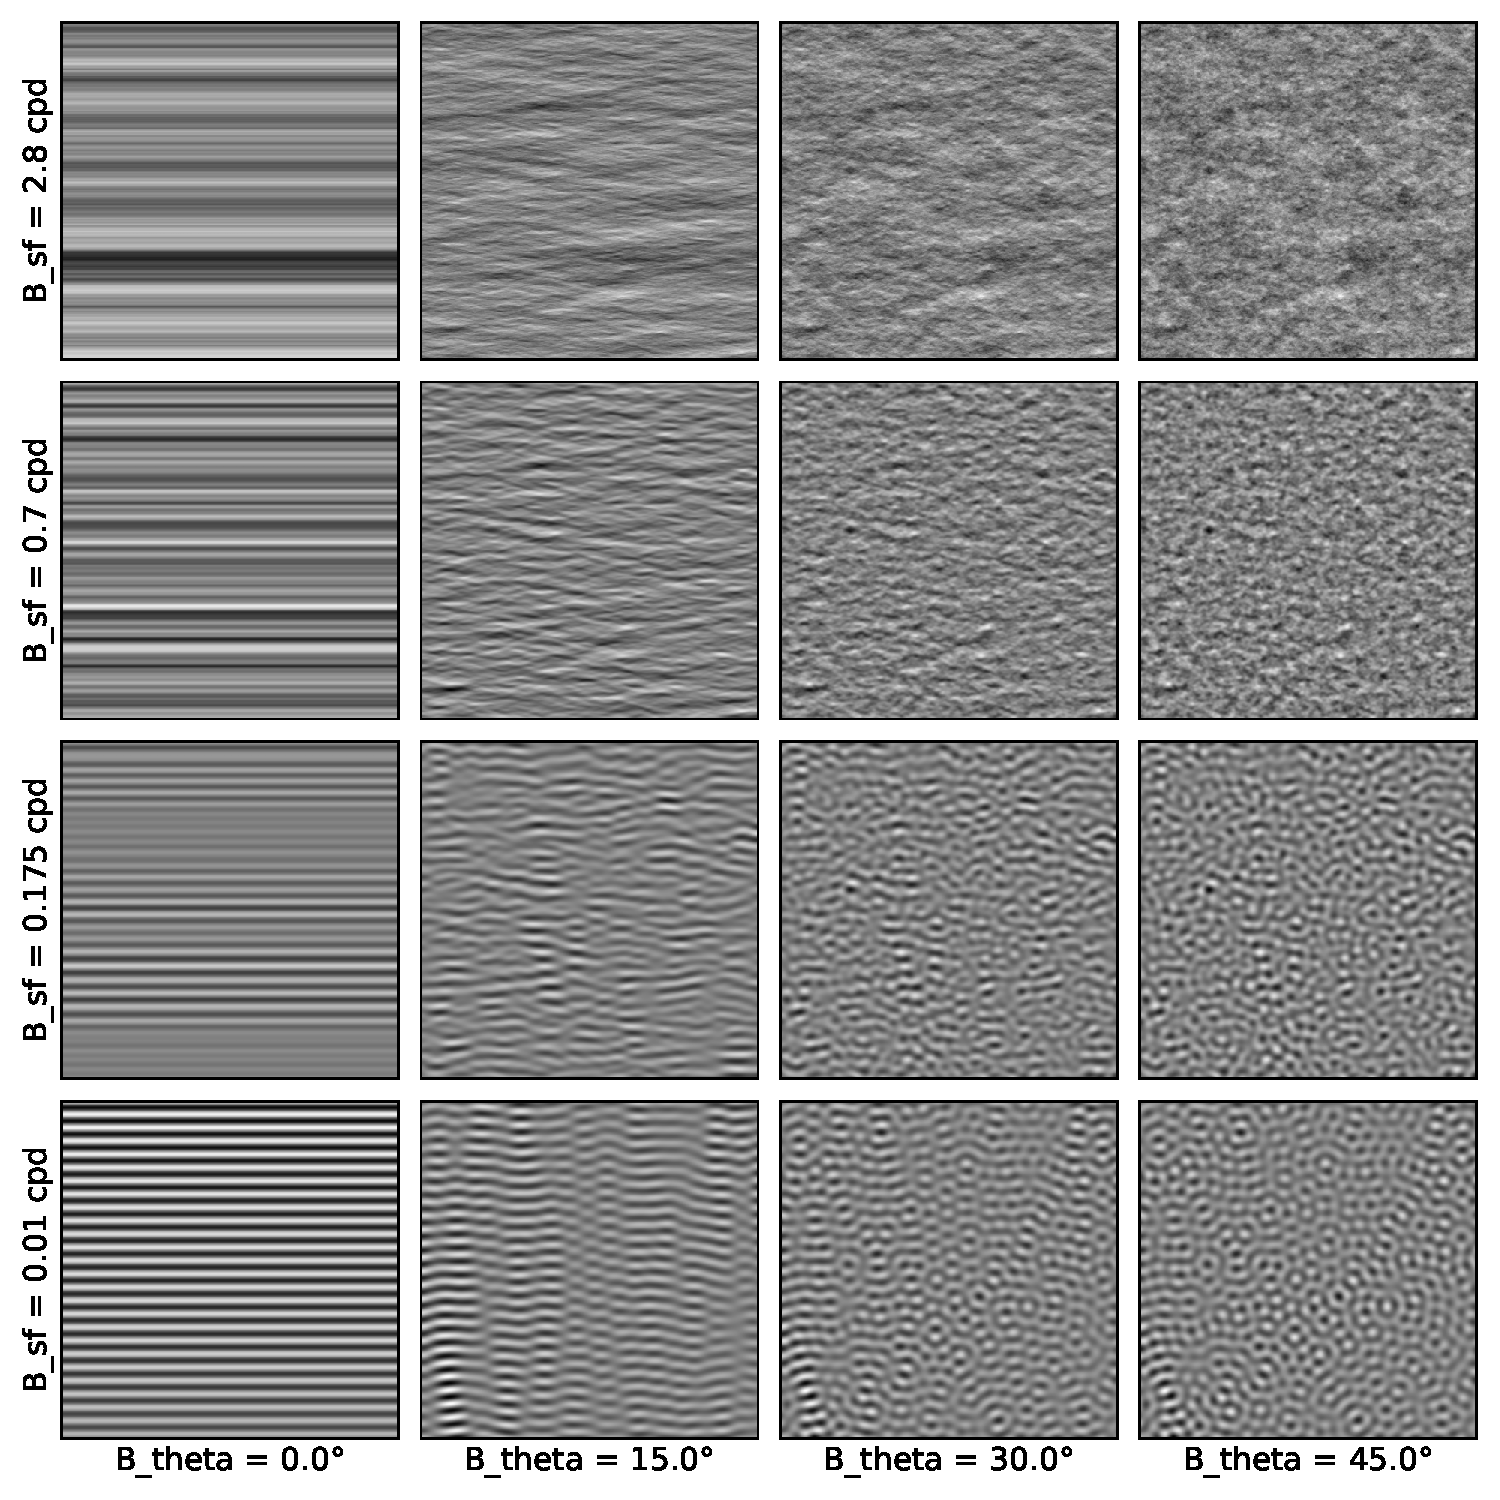
\includegraphics[width=\textwidth]{overview_of_stimuli.pdf}
                    \captionof{figure}{Motion-Clouds examples from sinusoidal grating (\textbf{C}) to pink noise (\textbf{B}), 2D noise (\textbf{A})and 1D noise (\textbf{D}).}
                \end{minipage}
            \end{tcolorbox}
        \end{minipage}
    \end{minipage} 
    \vspace{0.5cm}

    \begin{minipage}{\textwidth}
        \begin{minipage}{0.48\textwidth}
            \begin{tcolorbox}[
                enhanced,
                colframe=green!85!black!75,
                colback=white,
                arc=3mm,
                boxsep=5mm,
                boxrule=3pt,
                attach boxed title to top left={xshift=8mm,yshift=-3mm},
                boxed title style={
                    colback=white,
                    colframe=white,
                    sharp corners
                },
                coltitle=black,
                title=\textbf{\Large{Results : single neuron analysis}}
            ]
                \begin{minipage}{\textwidth}
                    \begin{center}
                        \begin{minipage}{\textwidth}
                            \center 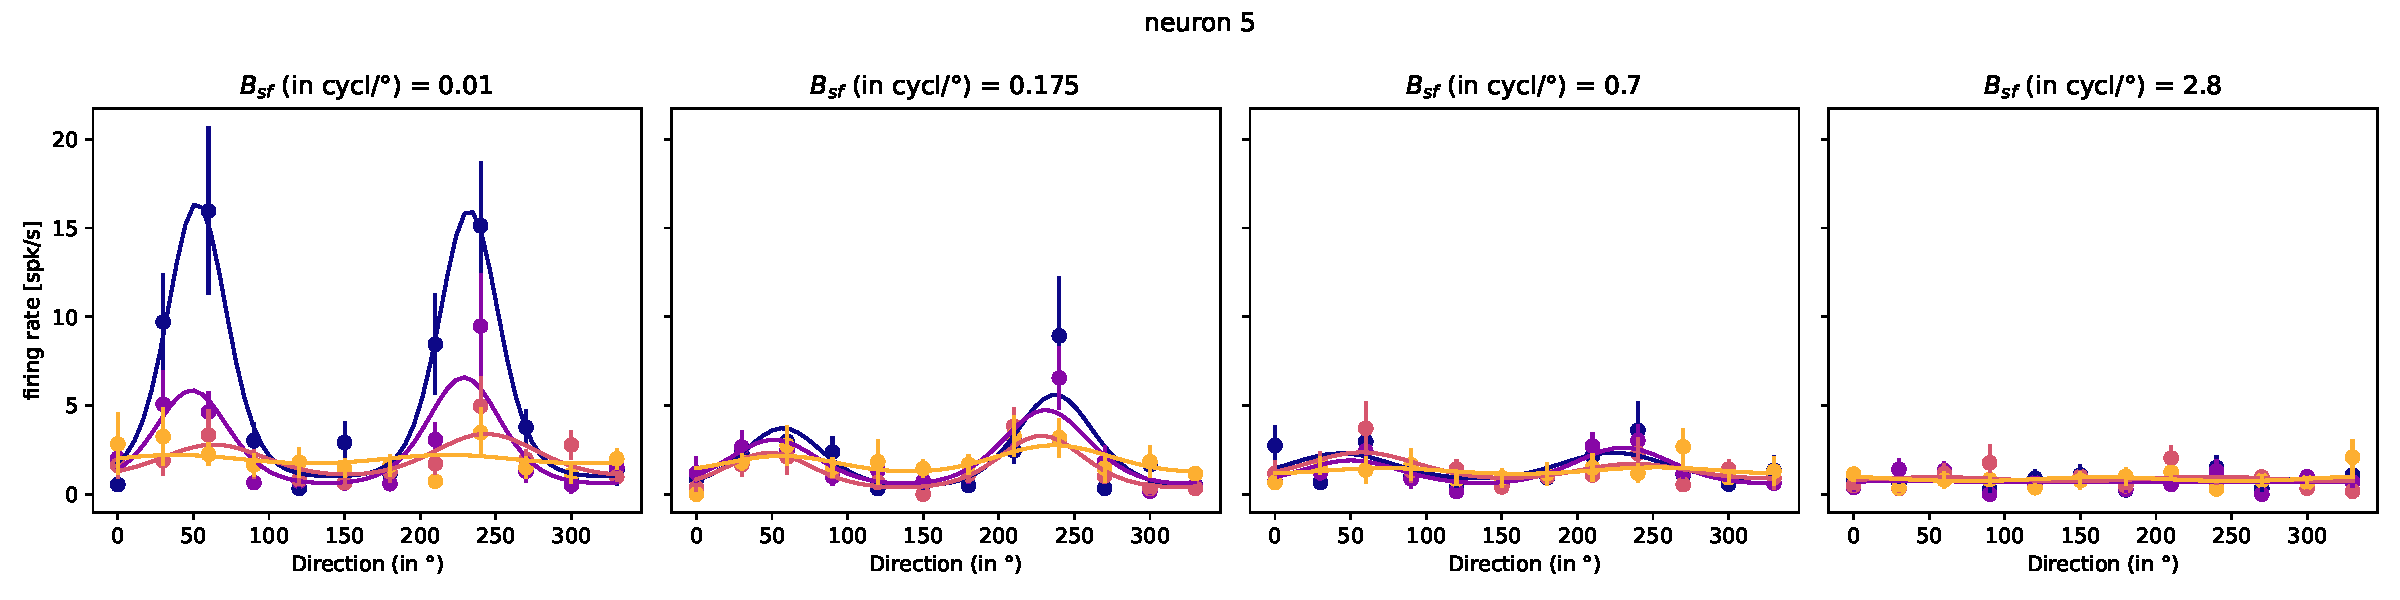
\includegraphics[width=0.97\textwidth]{part7g19_neuron-5_tc.pdf}
                        \end{minipage}
                        \vfill
                        \begin{minipage}{\textwidth}
                            \center 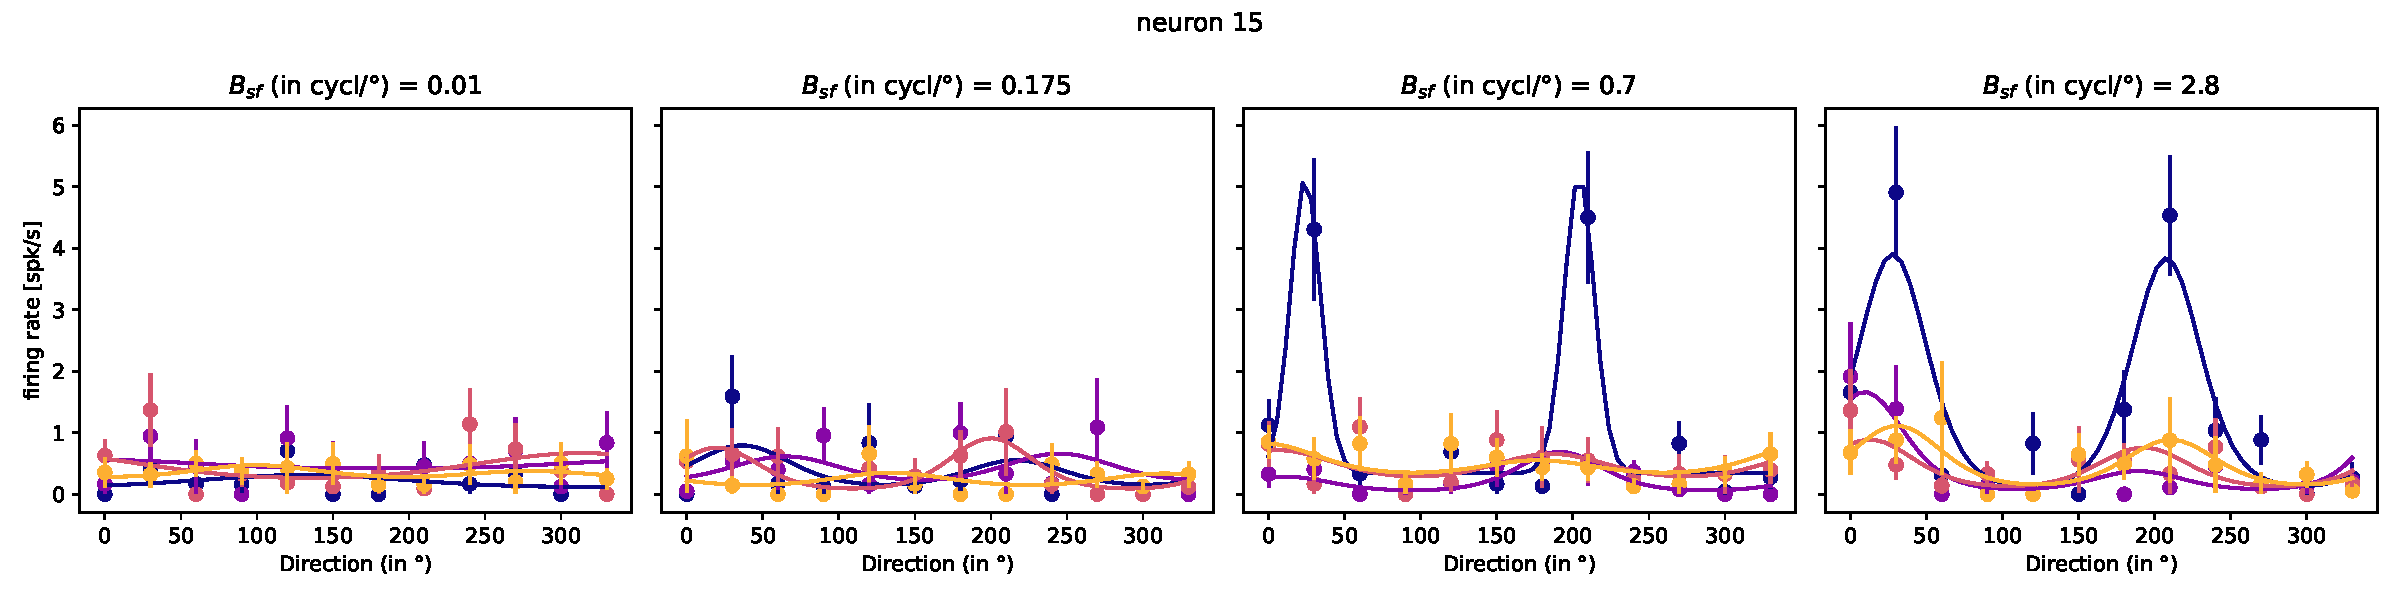
\includegraphics[width=0.97\textwidth]{part4g9_neuron-15_tc.pdf}
                        \end{minipage}
                        \vfill
                        \begin{minipage}{\textwidth}
                            \center 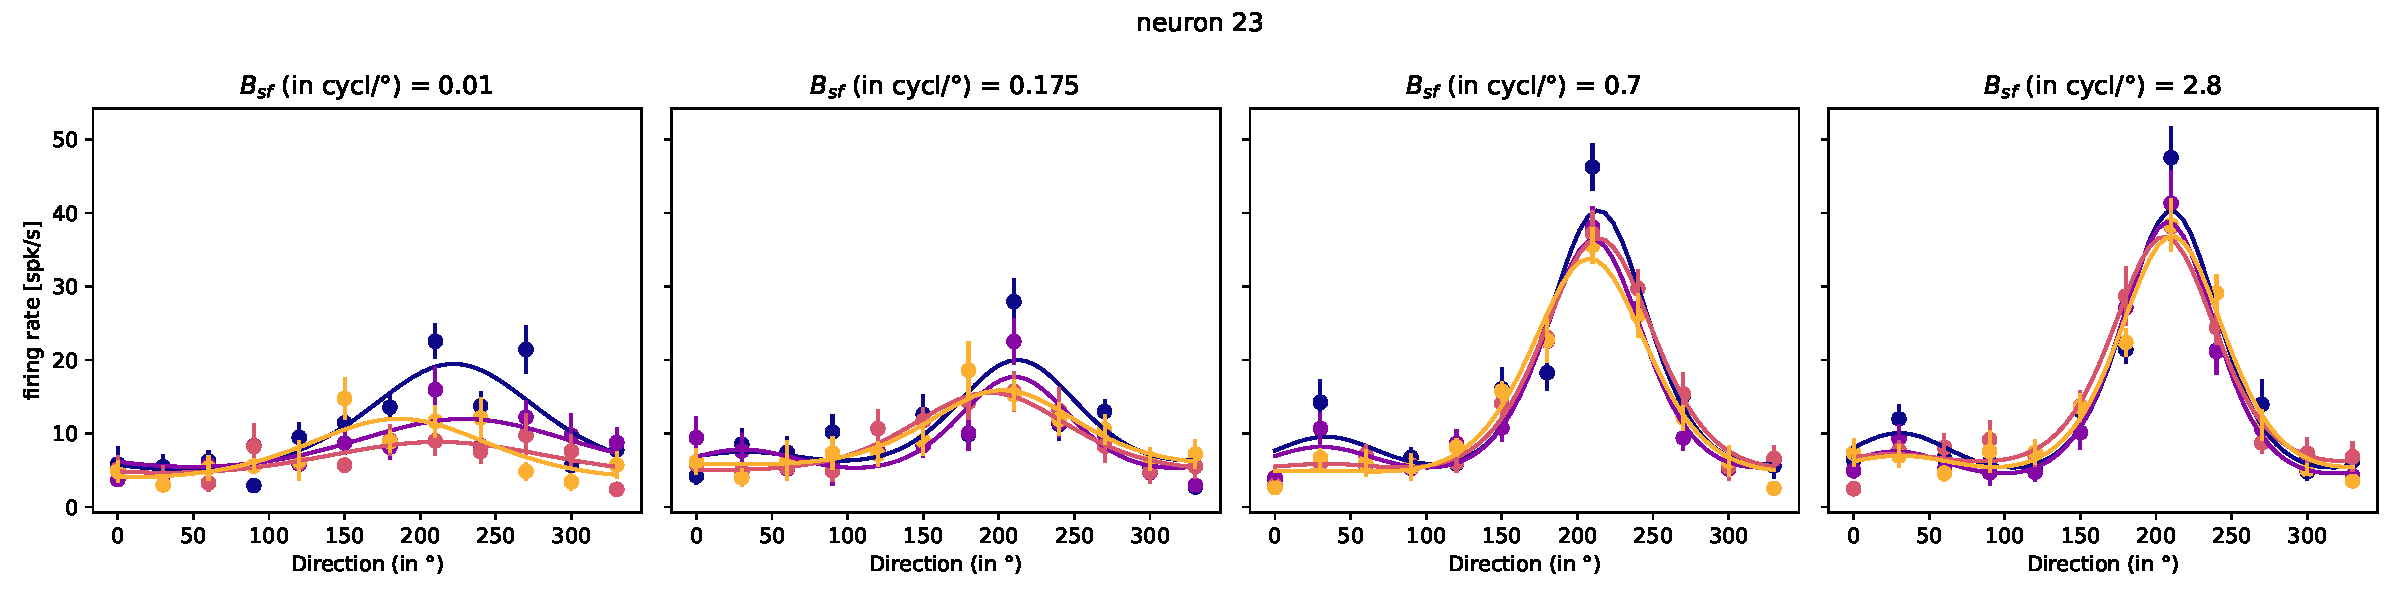
\includegraphics[width=0.97\textwidth]{part2g2_neuron-23_tc.pdf}
                        \end{minipage}
                    \end{center}
                    \vfill
                    \begin{minipage}{\textwidth}
                        \begin{center}
                            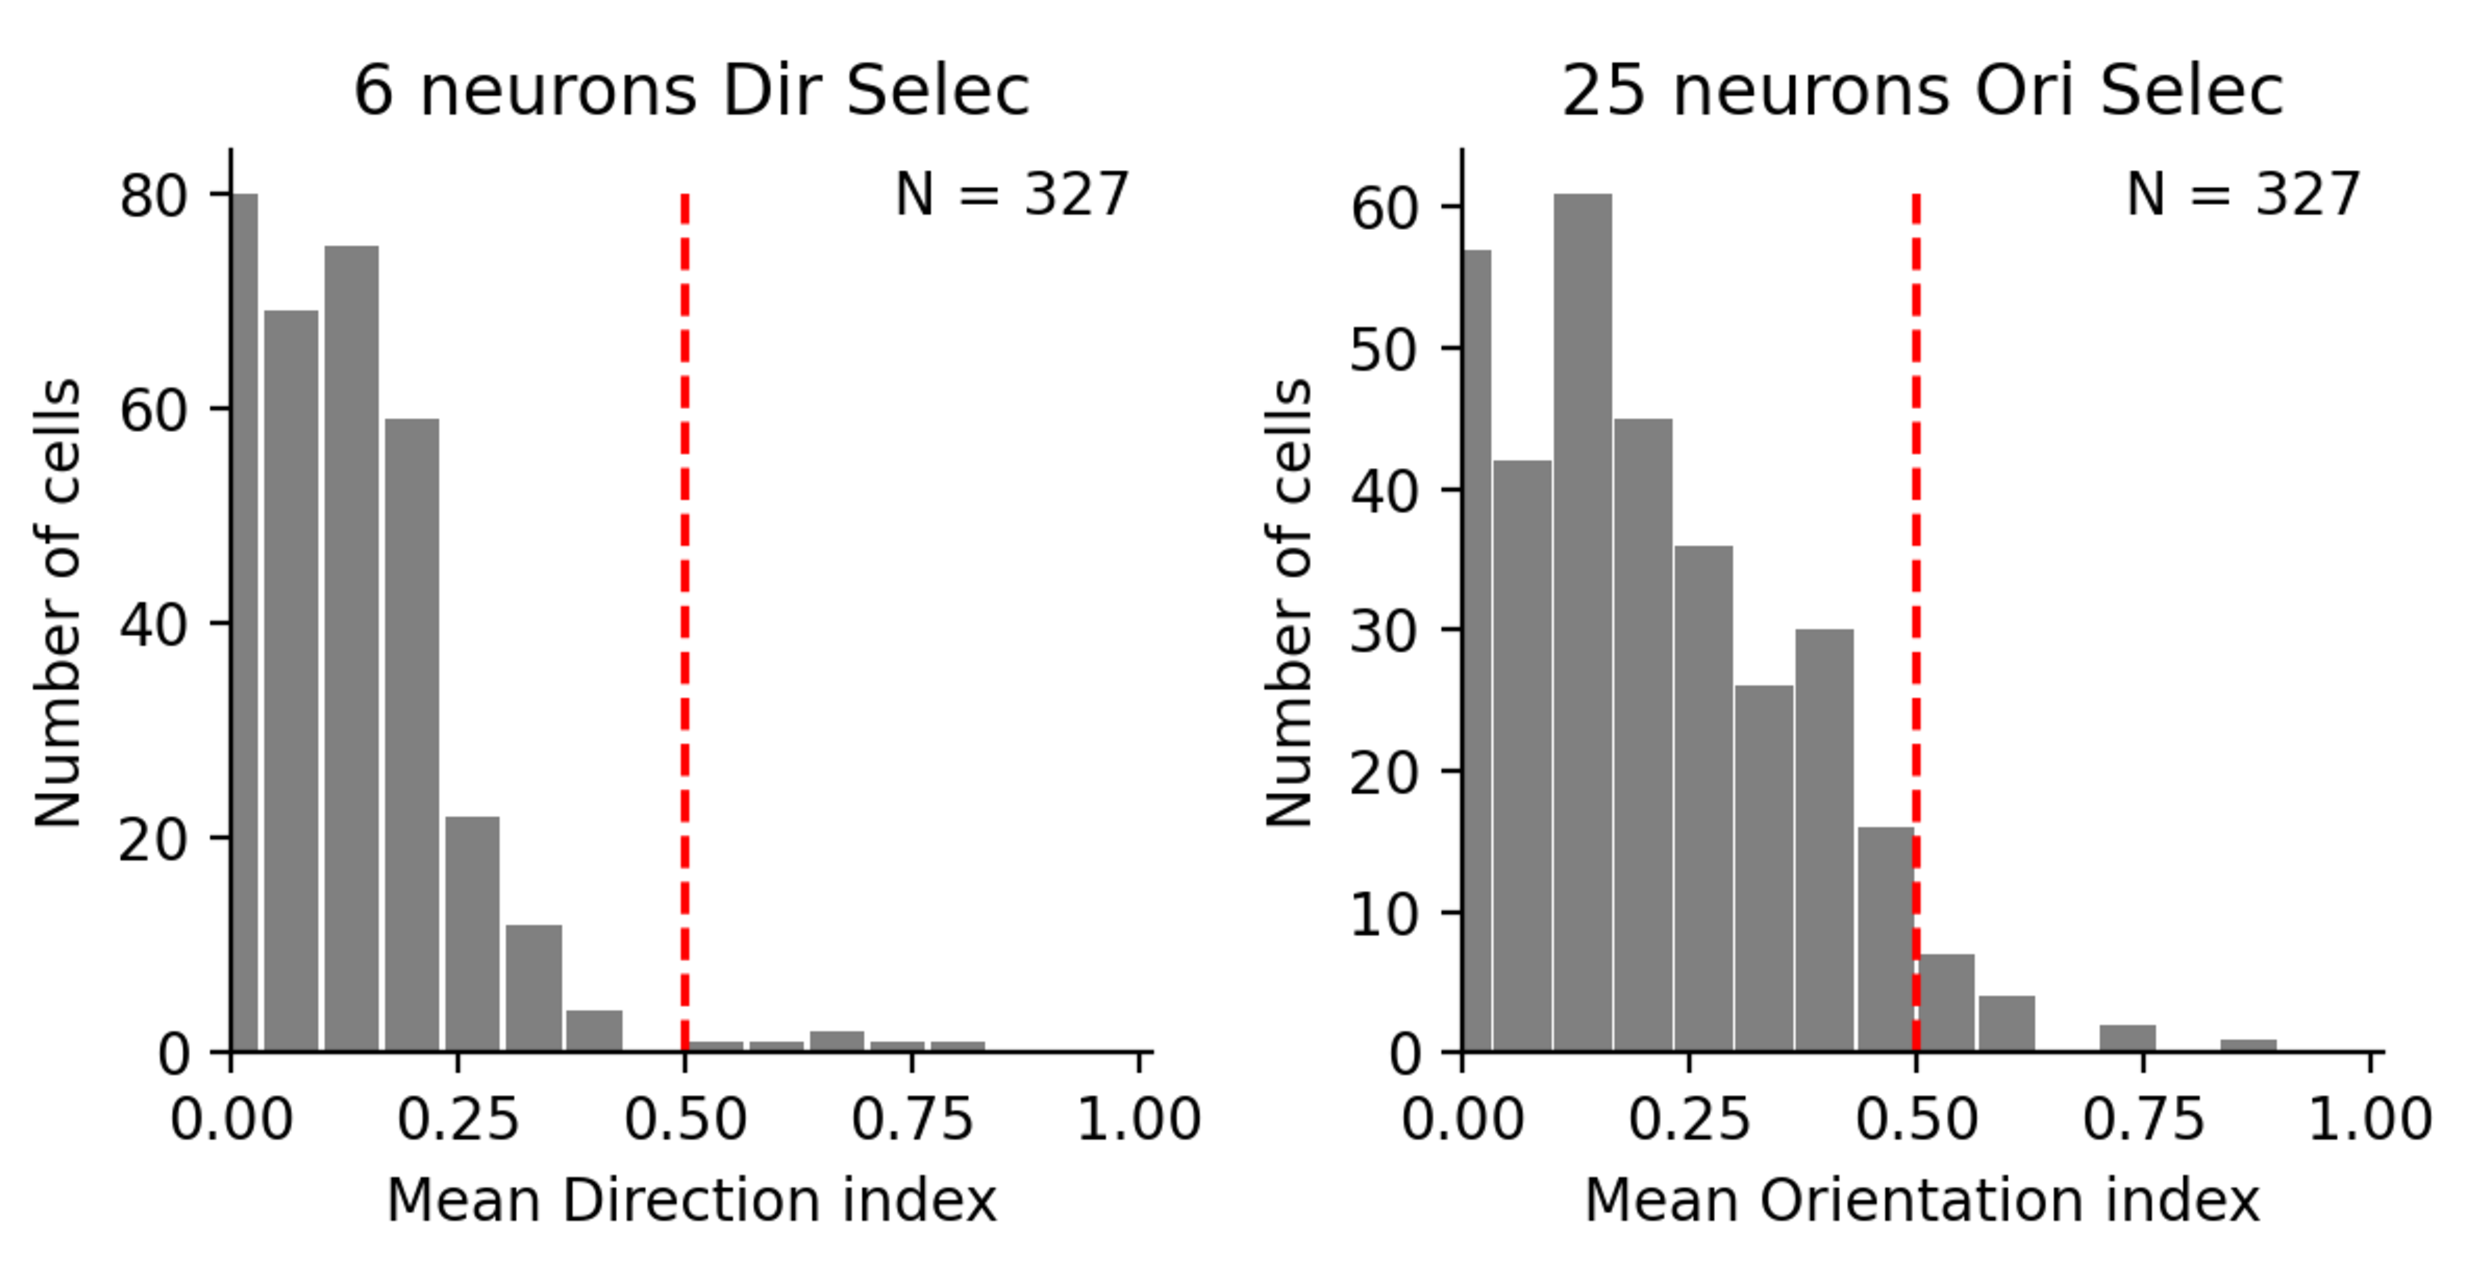
\includegraphics[width=0.49\textwidth]{pooling.pdf}
                            \hfill
                            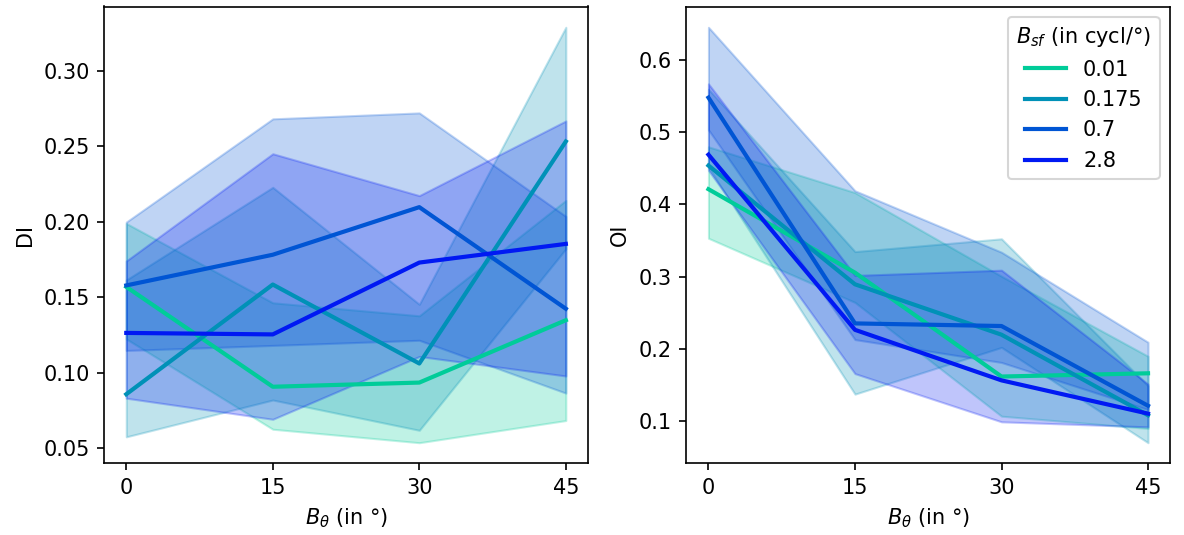
\includegraphics[width=0.49\textwidth]{OSI-DSI.pdf}
                        \end{center}
                    \end{minipage} 
                    % \captionof{figure}{Representative fitted tuning curves for different orientation and spatial frequency bandwidths. Distribution and modulation of orientation and direction selectivity indices (OI, DI) across bandwidth conditions.}
                \end{minipage} 
            \end{tcolorbox}
        \end{minipage}
        \hfill 
        \begin{minipage}{0.51\textwidth}
            \begin{tcolorbox}[ 
                enhanced,
                colframe=green!85!black!75, 
                colback=white,
                arc=3mm,
                boxsep=2mm,
                boxrule=3pt,
                attach boxed title to top left={xshift=8mm,yshift=-3mm}, 
                boxed title style={
                    colback=white, 
                    colframe=white,
                    sharp corners
                },
                coltitle=black,
                title=\textbf{\Large{Results : population decoding}}
            ]  
                \begin{minipage}{0.98\textwidth} % Decoding 
                    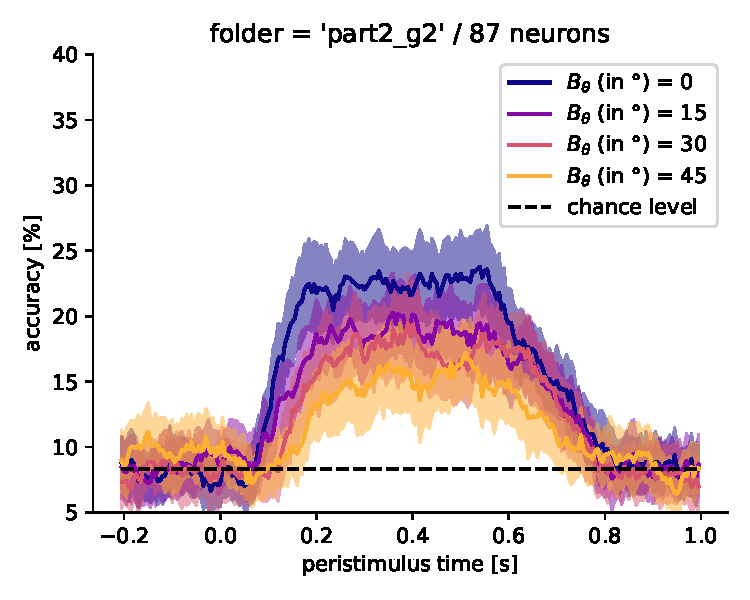
\includegraphics[width=0.32\textwidth]{part2_g2_theta_B_theta_Accuracy.pdf}
                    \hfill
                    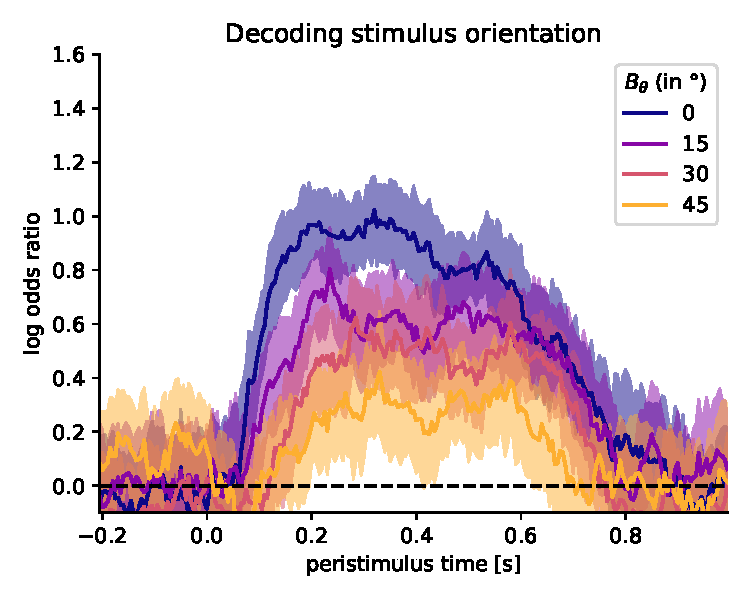
\includegraphics[width=0.32\textwidth]{part2_g2_ori_B_theta_Accuracy.pdf}
                    \hfill
                    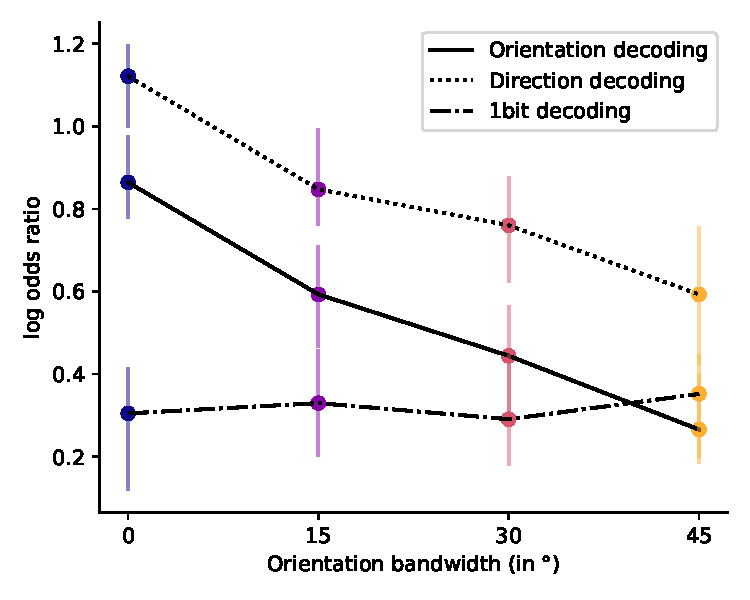
\includegraphics[width=0.32\textwidth]{part2_g2_B_theta_Mean_Accuracy.pdf}
                \end{minipage}

                \begin{minipage}{0.98\textwidth} % Decoding 
                    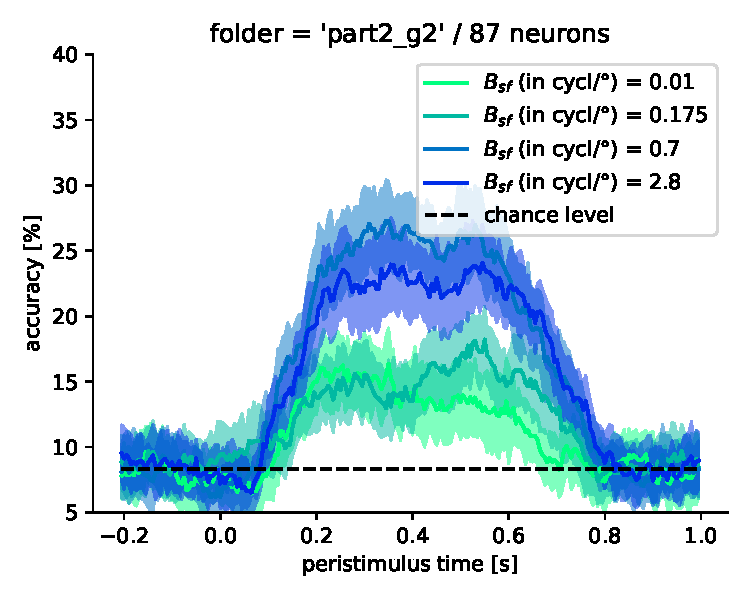
\includegraphics[width=0.32\textwidth]{part2_g2_theta_B_sf_Accuracy.pdf}
                    \hfill
                    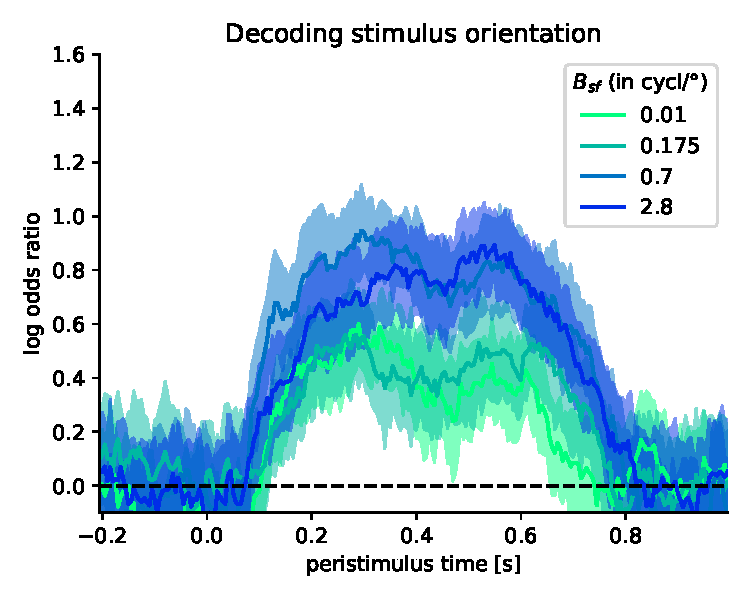
\includegraphics[width=0.32\textwidth]{part2_g2_ori_B_sf_Accuracy.pdf}
                    \hfill
                    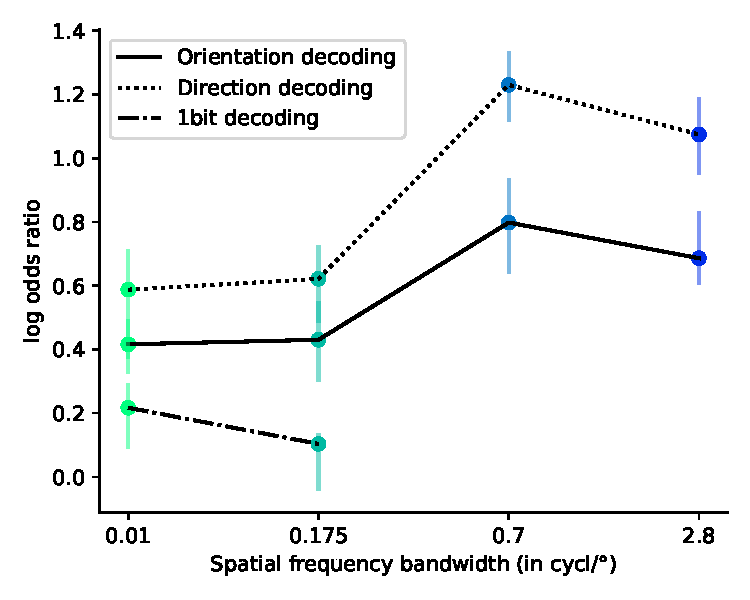
\includegraphics[width=0.32\textwidth]{part2_g2_B_sf_Mean_Accuracy.pdf}
                \end{minipage}
                
                \captionof{figure}{Direction ($\phi$), orientation ($\theta$)and direction bit decoding for different orientation and spatial frequency bandwidths ($B_\theta$, $B_{sf}$).}
            \end{tcolorbox}
            \vfill 
            \begin{tcolorbox}[
                enhanced,
                colframe=blue!60!white,
                colback=white,
                arc=3mm,
                boxsep=2mm,
                boxrule=3pt,
                attach boxed title to top left={xshift=8mm,yshift=-3mm},
                boxed title style={
                    colback=white,
                    colframe=white,
                    sharp corners
                },
                coltitle=black,
                title=\textbf{\Large{Perspectives}}
            ]
                Coupling decoding method and Motion-Clouds allow us to study how V1 population responses encode orientation and direction information by tiltrating the precision level in orientation and spatial frequency domains.
                In this context, MotionPlaids could offer an interesting next step to study how the brain combines oriented motion components, helping to disentangle orientation and direction contributions to population activity and to better understand how motion ambiguity is resolved in V1.
            \end{tcolorbox}
            \vfill
            \begin{tcolorbox}[
                enhanced,
                colframe=gray!60!white,
                colback=white,
                arc=3mm,
                boxsep=2mm,
                boxrule=3pt,
                attach boxed title to top left={xshift=8mm,yshift=-3mm},
                boxed title style={
                    colback=white,
                    colframe=white,
                    sharp corners
                },
                coltitle=black,
                title=\textbf{\large{References}}
            ]
                \printbibliography[heading=none]
            \end{tcolorbox}
        \end{minipage}    
    \end{minipage}
\end{document}